\chapter{Dérivabilité}
\paragraph{Définition}
$f:E \rightarrow \mathbb{R}, E$ est un voisinage de $x_0$.
f est \ul{derivable} en $x_0$ si $\frac{f(x)-f(x_0)}{x-x_0}$ admet une limite l quand x tend vers $x_0$ ($l \in \mathbb{R}$).
$\tau (x) = \frac{f(x)-f(x_0)}{x-x_0}$ est appelé le \ul{taux d'accroissement} de f en $x_0$. La limite de l (quand elle existe) est la dérivée de f en $x_0$, elle est notée $f'(x_0)$

\paragraph{Exemple} $
\begin{array}{rcll}
	f:&x&\mapsto &x^2 \\
	& \mathbb{R} &\rightarrow &\mathbb{R}
\end{array}$ $f'(1) =  ?$      $\begin{array}{rcl}
								\tau (x) & = & \frac{x^2 - x_0^2}{x-x_0} \\
										&=& \frac{(x-x_0)(x+x_0)}{x-x_0} \\
										\lim_{x \to x_0} x+x_0 &=& 2x_0 
								\end{array} $

\paragraph{Exemple 2} 
$
\begin{array}{rcll}
	f:&x&\mapsto &x^3 \\
	& \mathbb{R} &\rightarrow &\mathbb{R} 
\end{array}$

$\forall x \neq x_0, \begin{array}{rcl}
\tau (x) &=& \frac{x^3 - x_0^3}{x - x_0} \\
 &=& \frac{(x-x_0)(x^2+x.x_0+x_0^2)}{x-x_0}\\
\lim_{x\to x_0} x^2 + x.x_0+x_0^2 &=& 3x_0^2 
\end{array}$
~\\
$\forall x_0 \in \mathbb{R}, f'(x) = 3x_0^2$

\paragraph{Exemple 3}

$
\begin{array}{rcll}
	f:&x&\mapsto & \sqrt{x} \\
	& \mathbb{R}^+ &\rightarrow &\mathbb{R}
\end{array}$

$\forall x \neq x_0, x_0 \in \mathbb{R}^{+*} \begin{array}{rcl}
\tau (x) &=& \frac{\sqrt{x}-\sqrt{x_0}}{x-x_0} \\
			   &=&\frac{(\sqrt{x}-\sqrt{x_0})(\sqrt{x}+\sqrt{x_0})}{(x-x_0)(\sqrt{x}+\sqrt{x_0})} \\
	  &=& \frac{x-x_0}{(x-x_0)(\sqrt{x}+\sqrt{x_0})} \\
\lim_{x \to x_0} \tau (x) &=& \lim_{x \to x_0} \frac{1}{\sqrt{x}+\sqrt{x_0}} \\
						  &=& \frac{1}{2\sqrt{x_0}}
\end{array}$

\section{Interprétation géométrique} 
\begin{wrapfigure}[7]{r}{0pt}
	\begin{tikzpicture}
		\draw[->, thick] (-1, 0) -- (4, 0);
		\draw[->, thick] (0, -1) -- (0, 4);
		\draw[name path=courbe] (-1, 0.1) .. controls (1, 0.3) and (2, 1) .. (3, 3) node [above] {$D_{x_1}$};
		\node at (1, 0) [below] {$x_0$};
		\node at (2, 0) [below] {$x_1$};
		\path[name path=da] (1, 0) --(1, 3);
		\path[name path=db] (2, 0) --(2, 3);

		\draw[gray, dashed, name intersections={of=courbe and da}] (intersection-1) coordinate (i1) -- (1, 0);
		\draw[gray, dashed, name intersections={of=courbe and db}] (intersection-1) coordinate (i2) -- (2, 0);

		\getxy{\xa}{\ya}{i1}
		\draw[dashed, gray] (i1) -- (0, \ya) node [left, color=black] {$f(x_0)$};

		\getxy{\xb}{\yb}{i2};
		\draw[dashed, gray] (i2) -- (0, \yb) node [left, color=black] {$f(x_1)$};
		\draw[red] (-1, -0.5) -- (i1) -- (i2) -- (4, 3) node [above right] {Droite};

	\end{tikzpicture}
\end{wrapfigure}
$f'(x_0)$ est le coefficient directeur de la tangente du graphe de f en $(x_0,f(x_0))$

$\tau (x_1) = \frac{f(x_1)-f(x_0)}{x_1-x_0}$ est le coefficient de la droite passant par $P_{x_1}$ et $P_{x_0}$ avec $P_{x_1}$ du graph au point $x_1$, et $P_{x_0}$ celui de $x_0$
~\\
$y=\tau (x_1)(x-x_0) + f(x_0)$ avec $x_1 \in \mathbb{R}$

Quand x tend vers $x_0$, la droite $D_{x_1}$  "converge" vers la tangeante au graph de f au point ($x_0, f(x_0)$), d'équation :

$y = f'(x_0)(x-x_0)+f(x_0)$

\paragraph{Définition}
Si $\lim_{\substack{x \to x_0 \\ x < x_0}} \tau (x) = l^-, l^- \in \mathbb{R}$~\\
On dit que f est dérivable à gauche en $x_0$ et on note $f'_g(x_0) = l^-$

Si $\lim_{\substack{x \to x_0 \\ x > x_0}} \tau (x) = l^+, l^+ \in \mathbb{R}$~\\
f admet une dérivée à droite en $x_0$, que l'on note $f'_d(x_0) = l^+$

\paragraph{Théorème} $f:E \rightarrow \mathbb{R}, E$ un voisinage de $x_0$. f est dérivable en $x_0$ si et seulement si f est dérivable à droite et à gauche en $x_0$ et $f'_d(x_0) = f'_g(x_0)$

\paragraph{Remarque}
\begin{wrapfigure}[5]{l}{0pt}
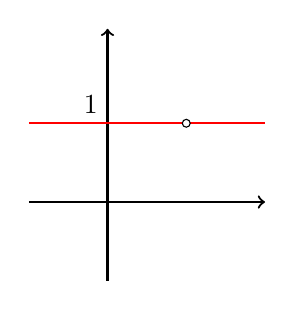
\begin{tikzpicture}
		\draw[->, thick] (-1, 0) -- (2, 0);
		\draw[->, thick] (0, -1) -- (0, 2.2);
		\draw[red, thick] (-1, 1) -- (2, 1);
		\draw[fill=white] (0, 1) node [above left] {1};
		\draw[fill=white] (1, 1) circle (0.05);
\end{tikzpicture}
\end{wrapfigure}
Cette fonction n'est pas dérivable en $1$, pourtant $f'_d(1) = f'_g(1)$, f doit donc alors être continue en $x_0$

\paragraph{Démonstration} f est dérivable en $x_0$, alors $\lim_{x \to x_0} \tau (x) = l \in \mathbb{R}$, cela signifie donc que $\begin{array} {rcl}
	\exists \delta > 0, |x-x_0| < \delta &\text{ donc }& |\tau (x) - l| < 1 \\
																						 & & l-1 \leq \tau (x) \leq l+1 \\
																				   & & l-1 \leq \frac{f(x) - f(x_0)}{x-x_0} \leq l+1 \end{array}$

	Si $x > x_0$, on obtient : \[ \begin{array}{rcl}
			(l-1)(x-x_0) \leq & f(x) - f(x_0) \leq & (l+1)(x-x_0) \\
			\lim_{x \to x_0} (l-1)(x-x_0) \leq & \lim_{x \to x_0}f(x) - f(x_0) \leq & \lim_{x \to x_0}(l+1)(x-x_0) \\
			0 \leq & \lim_{x \to x_0}f(x) - f(x_0) \leq & 0 \\
			  & \lim_{x \to x_0}f(x) - f(x_0) = 0 & \text{ par le théorème des gendarmes, et de même pour } x < x_0 \end{array} \]


\paragraph{Définition} $f:E \rightarrow \mathbb{R}$ 
f est dérivable sur l'intervalle ouvert $]a, b[$ si f est dérivable en tout point de $x_0 \in ]a, b[$
f est dérivable sur l'intervalle fermé $[a, b]$ si f est dérivable sur l'intervalle ouvert et à droite en a et à gauche en b.

\paragraph{Exemple} $x \to \sqrt{x}$ est dérivable sur $]0, +\infty[, [a, +\infty[ (a > 0)$ mais pas sur $[0, +\infty[$.

\section{Dérivabilité des prolongements de fonctions}
\paragraph{Proposition} $f:[a, b] \rightarrow \mathbb{R}, g [b, c] \rightarrow \mathbb{R}$ dérivable ~\\
On définit $\varphi : [a, c] \rightarrow \mathbb{R}$ par la formule $\varphi(x) \left\{ \begin{array}{rcl}
		f(x) & \text{ si } & x \in [a, b] \\
		g(x) & \text{ si } & x \in ]b, c] 
	\end{array}
	\right.$

	$\varphi $ est continue sur $[a, c]$ si \[\begin{array}{rcl} 
		\lim_{\substack{x \to b \\ x < b}}\varphi (x) &= \lim_{\substack{x \to b \\ x > b}}\varphi (x) &= \varphi(b) \\
		f(b) &= g(x) & = f(b) 
	\end{array}\]

		Si $\varphi$ est continue, $\varphi$ est dérivable sur $[a, c]$ si $f'_g(b) = g'_d(b)$

		\paragraph{Exercice} Trouver $\alpha$ et $\beta$ tels que $f:\mathbb{R} \rightarrow \mathbb{R}$ définie par 
		\[f(x) = 
			\left\{
				\begin{array}{rl}
					e^x +2, & \text{ si } x \leq 1 \\
					\alpha x + \beta & \text{ si } x > 1
				\end{array}
				\right.
			\]
			Soit dérivable sur $\mathbb{R}$. Comme $e^x +2$ et $\alpha x + \beta$ sont dérivable sur $\mathbb{R}$, le seul problème peut survenir en 1.
			Pour être dérivable, f doit être continue :
			$e^1 + 2 = \alpha + \beta$ et on doit avoir $f'_g(1) = e = f'_d(1) = \alpha$. $\alpha = e$ et $\beta = 2$

			\section{Opération usuelles} ~\\
			$f, g E \rightarrow \mathbb{R}, E$ voisinage de $x_0$.
			~\\
			f et g sont dérivable en $x_0$, alors :
			\begin{itemize}
				\item f+g est dérivable en $x_0$ et $(f+g)'(x_0) = f'(x)+g'(x)$
				\item f*g est dérivable en $x_0$ et $(f*g)'(x_0) = f'(x_0)*g(x_0)+f(x_0)*g'(x_0)$
				\item si $g(x_0) \neq 0$ $\frac{f}{g}$ est dérivable en $x_0$ et $(\frac{f}{g})'(x_0) = \frac{f'(x_0)*g(x_0)-f(x_0)*g'(x_0)}{g(x_0)^2}$
			\end{itemize}

			\paragraph{Démonstration} 
			Pour la somme : 
			\[\begin{array}{rcl}
				(f+g)(x) - (f+g)(x_0) &=& f(x)+g(x) - (f(x_0)+g(x_0)) \\
																							   &=& f(x) - f(x_0) + g(x) - g(x_0) \\
				\frac{(f+g)(x)-(f+g)(x_0)}{x-x_0} &=& \frac{f(x) - f(x_0)}{x_0} + \frac{g(x) - g(x_0)}{x-x_0}
		\end{array}\]

			Pour le produit :
			
			$\begin{array}{rcl}
				(f*g)(x) - (f*g)(x_0) &=& f(x)*g(x) - (f(x_0)*g(x_0)) \\
																							   &=& (f(x)-f(x_0))g(x) + f(x_0)g(x) - f(x_0)g(x_0) \\
																							   &=& (f(x)-f(x_0))g(x) + f(x_0)(g(x) -g(x_0))\\
				\frac{(f*g)(x)-(f*g)(x_0)}{x-x_0} &=& \frac{f(x) - f(x_0)}{x_0}g(x) + \frac{g(x) - g(x_0)}{x-x_0}f(x_0)
			\end{array}$
			~\\
			~\\
			Comme précédemment, $\lim_{x \to x_0}{g(x)} = g(x_0)$ car $g$ est continue en $x_0$

			\[\begin{array}{rcl}
					\frac{f}{g} &=& f . \frac{1}{g} \\
					(\frac{f}{g})' &=& f'.\frac{1}{g'} + f.(\frac{1}{g})'
				\end{array}
			\]

			\paragraph{Composition} $f:E \rightarrow F, g : F \rightarrow G, gof E \rightarrow G$ ~\\
			On suppose f dérivable en $x_0$, g dérivable en $f(x_0)$ alors $gof$ est dérivable en x et $(gof)'(x_0) = f'(x_0)\cdot g'(f(x_0))$
